\documentclass[tikz,border=10pt]{standalone}
\usepackage{tikz}
\usetikzlibrary{arrows.meta,positioning,shapes,calc}

\begin{document}
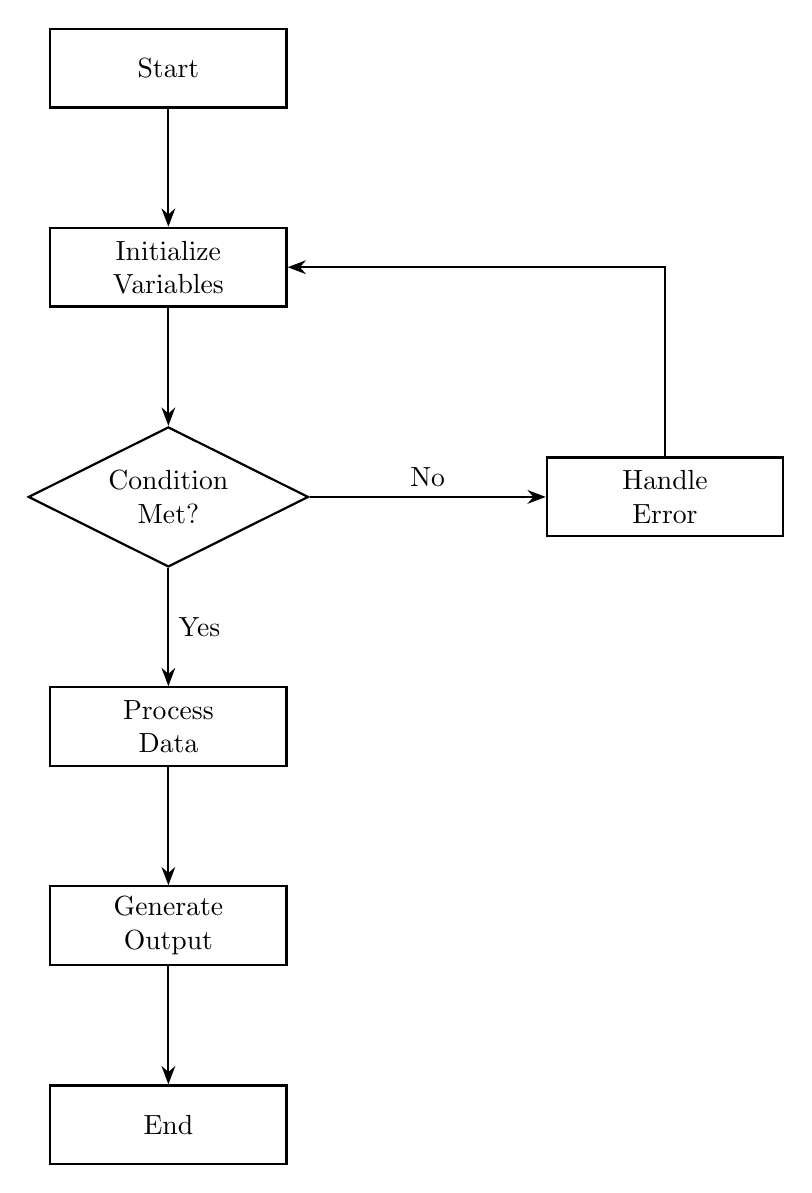
\begin{tikzpicture}[
    node distance=1.5cm,
    box/.style={rectangle, draw, thick, minimum width=3cm, minimum height=1cm, align=center},
    decision/.style={diamond, draw, thick, minimum width=3cm, minimum height=1cm, align=center, aspect=2},
    arrow/.style={-Stealth, thick}
]

% Nodes
\node[box] (start) {Start};
\node[box, below=of start] (init) {Initialize\\Variables};
\node[decision, below=of init] (check) {Condition\\Met?};
\node[box, below=of check] (process) {Process\\Data};
\node[box, right=3cm of check] (error) {Handle\\Error};
\node[box, below=of process] (output) {Generate\\Output};
\node[box, below=of output] (end) {End};

% Arrows
\draw[arrow] (start) -- (init);
\draw[arrow] (init) -- (check);
\draw[arrow] (check) -- node[right] {Yes} (process);
\draw[arrow] (check) -- node[above] {No} (error);
\draw[arrow] (error) |- (init);
\draw[arrow] (process) -- (output);
\draw[arrow] (output) -- (end);

\end{tikzpicture}
\end{document}
